% "Лаба"

\documentclass[a5paper,10pt, twoside]{article} % тип документа

\usepackage{hyperref}

\usepackage{import}


%  Русский язык

\import{../../headers/}{russian.tex}

% Математика

\import{../../headers/}{math.tex}

\usepackage{concmath, euler}
% Дефайны

\import{../../headers/}{my_defs.tex}

\graphicspath{{pics/}} % где лежат картинки

% Title Page
\title
{
	\hfill \break	\hfill \break
	\hfill \break	\hfill \break
  \hfill \break	\hfill \break
	Лабораторная работа 4.3.1.
	
	ИЗУЧЕНИЕ ДИФРАКЦИИ СВЕТА
}
\author{Державин Андрей, Б01-901}

\setcounter{secnumdepth}{0}

\begin{document}
	
\maketitle


\thispagestyle{empty} % выключаем отображение номера для этой страницы

\newpage

\tableofcontents % Вывод содержания

\newpage


\paragraph{Цель работы:}

	исследовать явления дифракции Френеля и Фраунгофера на щели, изучить влияние дифракции на 
	разрешающую способность оптических инструментовю.

\paragraph{В работе используются:}

	оптическая скамья, ртутная лампа, моно-
	хроматор, щели с регулируемой шириной, рамка с вертикальной ни-
	тью, двойная щель, микроскоп на поперечных салазках с микрометри-
	ческим винтом, зрительная труба.

\section{Теоритические сведения}

\subsection{Дифракция Френеля}
	Схема установки для наблюдения дифракции Френеля представле на на рис. \ref{img:scheme0}.
	Световые лучи освещают щель $S_2$ и испытывают на ней дифракцию. Дифракционная картина
	рассматривается с помощью микроскопа $\text{М}$, сфокусированного на некоторую плоскость
	наблюдения $\text{П}$.

	\begin{figure}[h]\label{img:scheme0}
		\center{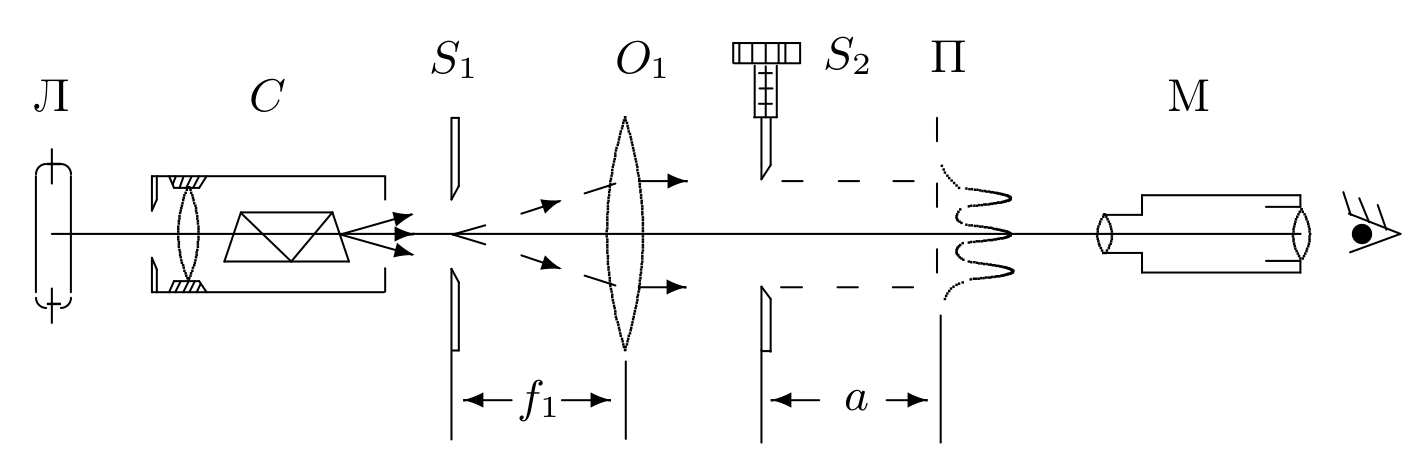
\includegraphics[width=1\linewidth]{scheme.png}}
		\caption{Схема установки для наблюдения дифракции Френеля}
	\end{figure}

	Щель $S_2$ освещается параллельным пучком монохроматического света с помощью коллиматора, 
	образованного объективом $O_1$ и щелью $S_1$, находящейся в его фокусе. На щель $S_1$ сфокусировано
	изображение спектральной линии, выделенной из спектра ртутной лампы $\text{Л}$ при помощи
	простого монохроматора $C$, в котором используется призма прямого зрения.

	Распределение интенсивности света в плоскости наблюдения $\text{П}$ проще всего рассчитывать с
	помощью зон	Френеля (для щели их иногда называют зонами Шустера). При освещении щели $S_2$
	параллельным пучком	лучей (плоская волна) зоны Френеля представляют собой полоски, параллельные
	краям щели (рис. \ref{img:zones}). Результирующая амплитуда в точке наблюдения определяется суперпозицией 
	колебаний от тех зон Френеля, которые не перекрыты створками щели. Графическое определение
	результирующей амплитуды производится с помощью векторной диаграммы -- спирали Корню. 
	Суммарная ширина $m$ зон Френеля $z m$ определяется соотношением
	\begin{equation}\label{eq:wide}
		z_m = \sqrt{a m \lambda}
	\end{equation}
	\
	где $a$ -- расстояние от щели до плоскости наблюдения (рис. \ref{img:scheme0}), а $\lambda$ --
	длина волны

	Вид наблюдаемой дифракционной картины определяется числом Френеля $\Phi$: квадрат числа Френеля

	\begin{displaymath}
		\Phi^2 = \frac{D}{\sqrt{a \lambda}}
	\end{displaymath}
	\
	-- это отношение ширины щели D к размеру первой зоны Френеля, т.е. число зон Френеля, которые
	укладываются на ширине щели. Обратную величину называют волновым параметром

	\begin{displaymath}
		p = \frac{1}{\Phi^2} = \frac{D}{\sqrt{a \lambda}}
	\end{displaymath}


	\begin{wrapfigure}{r}{0.4\linewidth} % обтекание текстом
		\label{img:zones}
		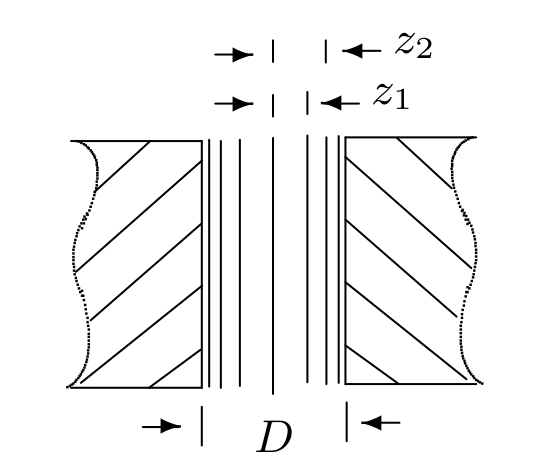
\includegraphics[width=\linewidth]{zones.png}
		\caption{Зоны Френеля в	плоскости щели}
	\end{wrapfigure}

	Дифракционная картина отсутствует, когда плоскость наблюдения $\text{П}$ совпадает с плоскостью
	щели: при $\Phi \rightarrow \infty$ мы имеем дело с геометрической оптикой. При небольшом
	удалении от щели, когда число Френеля $\Phi \gg 1$ (на щели укладывается огромное число зон),
	распределение интенсивности света за щелью также можно получить с помощью законов геометрической
	оптики (приближённо). Дифракционная картина в этом случае наблюдается только в узкой области на
	границе света и тени у краёв экрана.

	При последующем небольшом удалении от щели (или изменении ширины щели $S_2$ ) эти две группы
	дифракционных полос перемещаются практически независимо друг от друга. Каждая из этих групп
	образует картину дифракции Френеля на краю экрана. Распределение интенсивности при дифракции
	света на краю экрана может быть найдено с помощью спирали Корню.


	При дальнейшем увеличении расстояния $a$ (или уменьшении ширины	щели $S_2$ ) обе системы
	дифракционных полос постепенно сближаются и, наконец, при $\Phi \gtrsim 1$ накладываются друг на
	друга. Распределение интенсивности в плоскости наблюдения в этом случае определяется числом
	зон Френеля, укладывающихся на полуширине щели. Если это число равно $m$, то в поле зрения
	наблюдается $n = m - 1$ тёмных полос. Таким образом, по виду дифракционной картины можно оценить число
	зон Френеля на полуширине щели.
	
\subsection{Дифракция Фраунгофера на щели}

	Картина дифракции резко упрощается, когда ширина щели становится значительно меньше ширины первой
	зоны Френеля, т.е. если

	\begin{equation}\label{eq:frenele}
		D \gg \sqrt{a \lambda} \text{ или } \Phi \gg 1
	\end{equation}

	Это условие всегда выполняется при достаточно большом расстоянии a от щели до плоскости наблюдения.
	Дифракционную картину, наблюдаемую в этом случае, принято называть дифракцией Фраунгофера.
	Исследование такой дифракционной картины заметно облегчается, потому что упрощаются фазовые
	соотношения. Это поясняет рис. 3. При выполнении условия \eqref{eq:frenele} разность хода между
	крайними лучами, приходящими от щели в точку наблюдения $P$ , с хорошим приближением можно
	вычислять по формуле

	\begin{equation}\label{eq:delta}
		\delta = r_2 - r_1 \approx D \sin \Theta \approx D \cdot \Theta
	\end{equation}

	Здесь предполагается, что дифракционный угол $\Theta$ достаточно мал, так что 
	$\sin \Theta \approx \Theta$. Формула \eqref{eq:delta} справедлива при условии $\delta \ll \lambda / 2$.
	Можно показать, что это условие эквивалентно условию \eqref{eq:frenele}

	\begin{figure}[h]\label{img:scheme1}
		\center{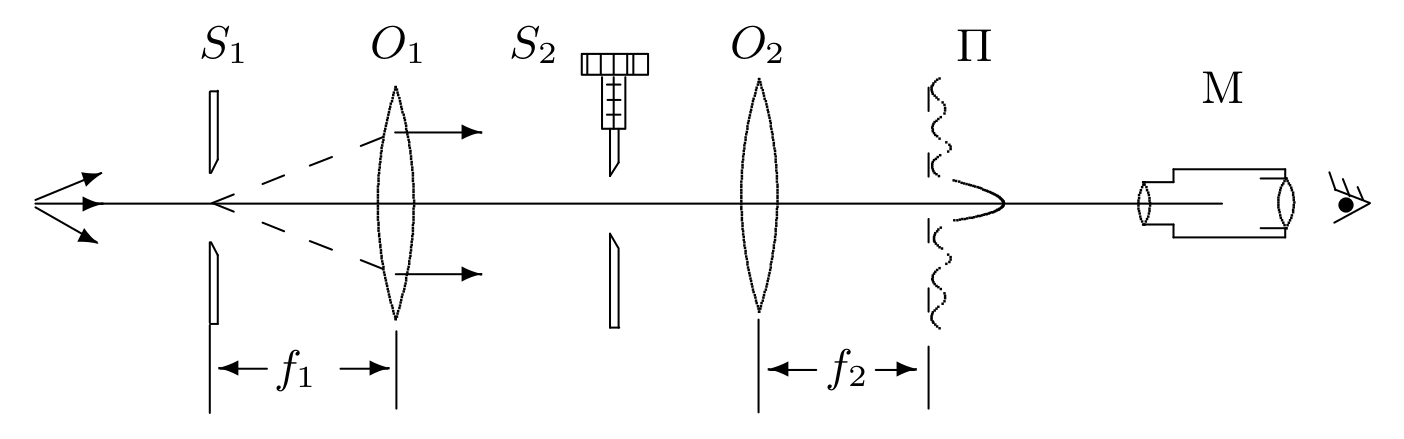
\includegraphics[width=1\linewidth]{scheme1.png}}
		\caption{Схема установки для наблюдения дифракции Фраунгофера на щели}
	\end{figure}


	Дифракцию Френеля и Фраунгофера можно наблюдать на одной и той же установке (рис. \ref{img:scheme0}).
	Однако при обычных размерах установки дифракция Фраунгофера возникает только при очень узких щелях.
	Например, при $a \approx 20-40$ см и $\lambda \approx 5 \cdot 10^{-5}$ см получаем $D \ll 0.3$ см.
	Поскольку работать с такими тонкими щелями неудобно, для наблюдения дифракции Фраунгофера к схеме,
	изображённой на рис. \ref{img:scheme0} добавляется объектив $O_2$ (рис. \ref{img:scheme1}).

	\begin{wrapfigure}{r}{0.4\linewidth} % обтекание текстом
		\label{img:phase}
		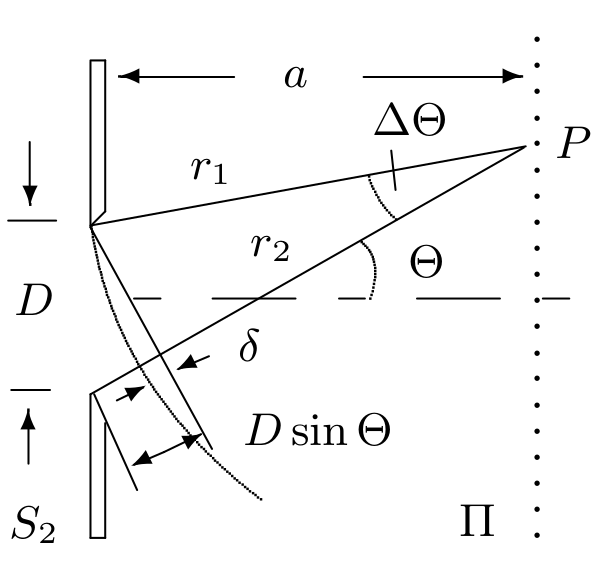
\includegraphics[width=\linewidth]{phase.png}
		\caption{К фазовым соотн. при дифр. Фраунгофера}
	\end{wrapfigure}

	Дифракционная картина наблюдается здесь в фокальной плоскости объектива $O_2$. Каждому значению
	угла $\Theta$ соответствует в этой плоскости точка, отстоящая от оптической оси на расстоянии

	\begin{equation}\label{eq:dist}
		X = f_2 \tg \Theta \approx f_2 \Theta
	\end{equation}

	Поскольку объектив не вносит дополнительной разности хода щели между интерферирующими лучами
	(таутохронизм), в его фокальной плоскости наблюдается неискажённая дифракционная картина 
	Фраунгофера. Эта картина соответствует бесконечно удалённой плоскости наблюдения. Распределение
	интенсивности в дифракционной картине Фраунгофера представлено на рис. \ref{img:phase}.

	\begin{wrapfigure}{r}{0.4\linewidth} % обтекание текстом
		\label{img:dist}
		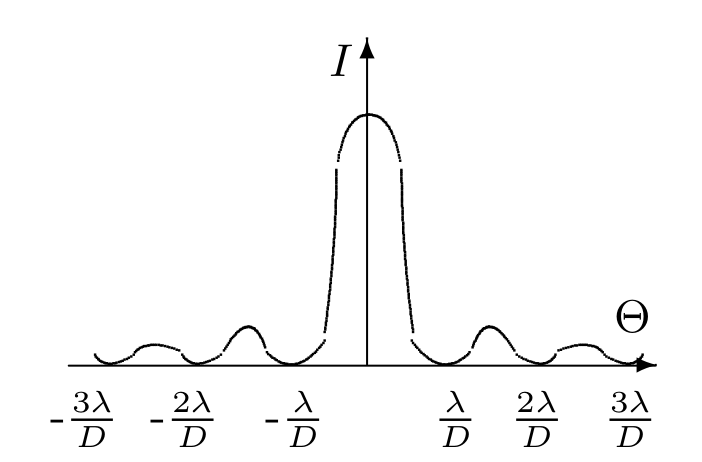
\includegraphics[width=\linewidth]{dist.png}
		\caption{Зоны Френеля в	плоскости щели}
	\end{wrapfigure}

	Поскольку при $\Theta = 0$ разность хода между любой парой лучей равна нулю, в центре поля зрения
	наблюдается дифракционный максимум (светлая полоса). Первый минимум (первая тёмная полоса) 
	соответствует, очевидно, такому значению дифракционного угла $\Theta_1$, при котором
	в точке наблюдения разность хода пробегает все возможные значения от нуля до $2 \pi$.
	Рассуждая аналогичным образом, можно определить угловую координату $\Theta_m$
	любой тёмной полосы. Для малых углов

	\begin{equation}\label{eq:ang}
		m \lambda = D \cdot \Theta
	\end{equation}

	Расстояние $X_m$ тёмной полосы от оптической оси объектива $O_2$ пропорционально фокусному
	расстоянию $f_2$. Из \eqref{eq:dist} и \eqref{eq:ang} следует

	\begin{equation}\label{eq:dist_m}
		X_m = f_2 \cdot m \frac{\lambda}{D}
	\end{equation}

	Из \eqref{eq:dist_m} видно, что при малых углах минимумы эквидистантны, а расстояния $\Delta X$
	между минимумами обратно пропорциональны ширине $D$ щели $S_2$.

\subsection{Дифракция Фраунгофера на двух щелях}
    \import{src/}{c.tex}

\subsection{Влияние дифракции на разрешающую способность оптического инструмента}
    \import{src/}{d.tex}

\section{Ход работы}

\subsection{Дифракция Френеля}

Подготавливаем приборы к работе, а затем, добившись наибольшей чёткости дифракционной картины, снова 
находим резкое изображение щели.

Приближая микроскоп к щели, снимаем зависимость координаты микроскопа от числа $n$ наблюдаемых тёмных 
полос.

Измеряем ширину $D$ щели $S_2$ , используя микрометрический винт поперечных салазок микроскопа.

Сравниваем размер зон Френеля с измеренной шириной $D$ щели $S_2$ . Для этого рассчитываем величину
$2 z m$ по формуле \eqref{eq:wide} 
и постройте график $2 z m = f(m)$. Отложите на графике величину $D$.
Длина волны зелёной линии ртути $\lambda$ = 5461 \AA.

\subsection{Дифракция Фраунгофера на щели}

Помещаем щель $S_2$ между линзами и наблюдаем дифракционную картинку. Измеряем с помощью винта 
поперечного перемещения микроскопа координаты $X_m$ нескольких дифракционных минимумов 
(от $-m$ до $+m$). Определите ширину $D$ щели $S_2$.

По углу наклона прямой определяем среднее расстояние $\Delta X$ между соседними минимумами;
рассчитываем ширину щели $D$ по формуле \eqref{eq:dist_m}.

\subsection{Дифракция Фраунгофера на двух щелях}

Заменяем в установке (рис. \ref{img:scheme1}) входную щель $S_1$ щелью с микрометрическим винтом.
Ставим между линзами экран Э с двойной щелью. В области главного дифракционного максимума должна 
появиться система равноотстоящих тёмных и светлых полос.

Определяем расстояние $\delta x$ между минимумами по результатам измерений, рассчитываем величину 
$d$ по формуле \eqref{eq:fraundx}. Рассчитываем число полос внутри главного максимума по формуле 
\eqref{eq:intnum}

\subsection{Влияние дифракции на разрешающую способность оптического инструмента}

Собираем схему согласно рис. \ref{img:fraunres}. Уменьшая ширину щели, наблюдаем за ухудшением 
качества изображения. Подберите ширину щели $S_2$ так, чтобы изображения обеих щелей почти сливались, 
но всё-таки ещё воспринимались раздельно.

\end{document} % конец документа
